\addcontentsline{toc}{section}{Introduction}
\section*{Introduction}

Les data warehouses et les lacs de données sont les référentiels de données centraux les plus couramment utilisés par la plupart des organisations axées sur les données aujourd'hui, chacun avec ses propres forces et compromis. D'une part, alors que les data warehouses permettent aux entreprises d'organiser des ensembles de données historiques à utiliser dans la Business Intelligence (BI) et l'analyse, ils deviennent rapidement plus coûteux à mesure que les ensembles de données augmentent en raison de l'utilisation combinée des ressources de calcul et de stockage. De plus, les data warehouses ne peuvent pas gérer la nature variée des données (structurées, non structurées et semi-structurées) observées aujourd'hui.

Dans ce chapitre, nous explorerons les principales caractéristiques de Delta Lake, son fonctionnement et pourquoi il s'agit d'un bon choix pour le traitement du Big Data. Nous fournirons également des exemples d'utilisation de Delta Lake avec d'autres outils de Big Data, tels que Spark et Trino, plus loin dans ce rapport.
\section{Définition}
Delta Lake est une couche de stockage open source construite au-dessus d'un lac de données qui confère fiabilité et transactions ACID (atomicité, cohérence, isolation et durabilité). Il permet une architecture de données continue et simplifiée pour les organisations. Un lac de données stocke les données au format Parquet et permet une architecture de données Lakehouse, qui aide les organisations à créer un système de données unique et continu qui combine les meilleures fonctionnalités de l'entrepôt de données et du lac de données tout en prenant en charge le traitement en continu et par lots.

\section{Comment fonctionne Delta Lake}
Un Delta Lake permet la construction d'une data lakehouse. Les datalakehouses courantes incluent Databricks Lakehouse et Azure Databricks. Cette architecture de données continue permet aux organisations d'exploiter les avantages des data warehouses et des lacs de données avec une complexité et des coûts de gestion réduits. Voici quelques façons dont Delta Lake améliore l'utilisation des data warehouses et des lacs:
\begin{itemize}
    \item \textbf{Permet une architecture Lakehouse:} Delta Lake permet une architecture de données continue et simplifiée qui permet aux organisations de gérer et de traiter d'énormes volumes de données en continu et par lots sans les tracas de gestion et d'exploitation liés à la gestion séparée du streaming, des data warehouses et des lacs de données.
    \item \textbf{Permet une gestion intelligente des données pour les lacs de données:} Delta Lake offre une gestion efficace et évolutive des métadonnées, qui fournit des informations sur les volumes de données massifs dans les lacs de données. Grâce à ces informations, les tâches de gouvernance et de gestion des données se déroulent plus efficacement.
    \item \textbf{Application du schéma pour une meilleure qualité des données:} Étant donné que les lacs de données n'ont pas de schéma défini, il devient facile pour les données mauvaises/incompatibles d'entrer dans les systèmes de données. La qualité des données est améliorée grâce à la validation automatique du schéma, qui valide la compatibilité DataFrame et table avant les écritures.
    \item \textbf{Permet la transaction ACID:} La plupart des architectures de données organisationnelles impliquent de nombreux mouvements ETL et ELT entrant et sortant du stockage de données, ce qui l'ouvre à plus de complexité et d'échecs aux points d'entrée des nœuds. Delta Lake garantit la durabilité et la persistance des données pendant l'ETL et d'autres opérations de données. Delta Lake capture toutes les modifications apportées aux données pendant les opérations de données dans un journal des transactions, garantissant ainsi l'intégrité et la fiabilité des données pendant les opérations de données.
\end{itemize}

\section{Diagramme d'architecture du Delta Lake}
\begin{flushleft}
Delta Lake est une amélioration de l'architecture lambda dans laquelle le traitement par flux et par lots se produit en parallèle et les résultats fusionnent pour fournir une réponse à la requête. Cependant, cette méthode signifie plus de complexité et de difficulté à maintenir et à exploiter à la fois les processus en continu et par lots. Contrairement à l'architecture lambda, Delta Lake est une architecture de données continues qui combine des flux de travail en continu et par lots dans un magasin de fichiers partagé via un pipeline connecté.
\end{flushleft}

Le fichier de données stocké comporte trois couches, les données s'affinant au fur et à mesure qu'elles progressent en aval dans le flux de données:

\begin{enumerate}
\item[$\bullet$] \textbf{Bronze tables:} Cette table contient les données brutes ingérées à partir de plusieurs sources telles que les systèmes Internet des objets (IoT), les fichiers CRM, RDBMS et JSON.
\item[$\bullet$] \textbf{Silver tables:} Cette couche contient une vue plus raffinée de nos données après avoir subi des processus de transformation et d'ingénierie de fonctionnalités.
\item[$\bullet$] \textbf{Gold tables:} Cette couche finale est souvent mise à la disposition des utilisateurs finaux dans les rapports et l'analyse BI ou utilisée dans les processus d'apprentissage automatique.
\end{enumerate}

\begin{figure}[htbp]
\centering
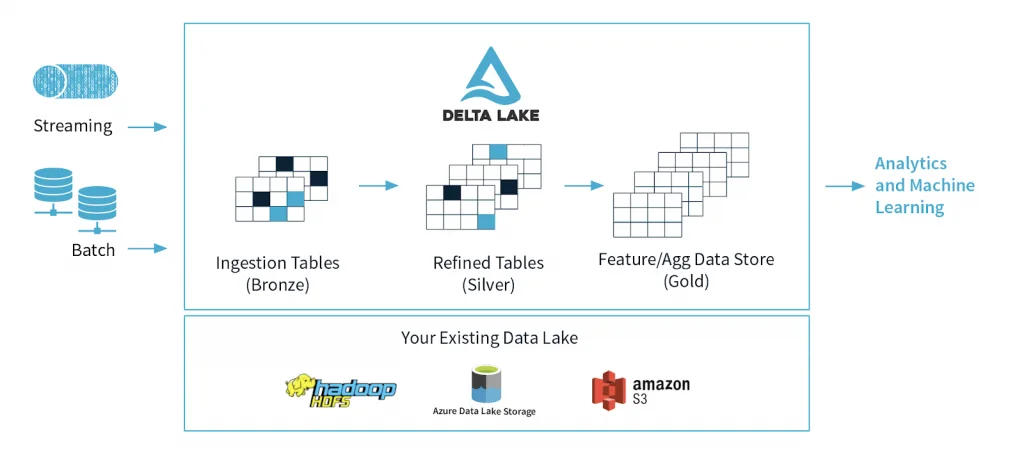
\includegraphics[width=\linewidth]{images/delta_lake_architecture.png}
\caption{Architecture multi-sauts de Delta Lake}\label{fig:delta-lake-architecture}
\end{figure}

\section{Principaux avantages et caractéristiques de Delta Lake}
\begin{itemize}
    \item[\textbullet] \textbf{Pistes d'audit et historique:}Dans Delta Lake, chaque écriture existe en tant que transaction et est enregistrée en série dans un journal des transactions. Par conséquent, toutes les modifications ou validations apportées au journal des transactions sont enregistrées, laissant une trace complète à utiliser dans les audits historiques, la gestion des versions ou à des fins de voyage dans le temps. Cette fonctionnalité de Delta Lake permet de garantir l'intégrité et la fiabilité des données pour les opérations de données d'entreprise.
    \item[\textbullet] \textbf{Voyager dans le temps et versionner les données:} Étant donné que chaque écriture crée une nouvelle version et stocke l'ancienne version dans le journal des transactions, les utilisateurs peuvent afficher/restaurer les anciennes versions de données en fournissant l'horodatage ou le numéro de version d'une table ou d'un répertoire existant à l'API de lecture Sparks\@. À l'aide du numéro de version fourni, Delta Lake construit ensuite un instantané complet de la version avec les informations fournies par le journal des transactions. Les retours en arrière et la gestion des versions jouent un rôle essentiel dans l'expérimentation de l'apprentissage automatique, où les scientifiques des données modifient de manière itérative les hyperparamètres pour former des modèles et peuvent revenir aux modifications si nécessaire.
    \item[\textbullet] \textbf{Unifie le traitement par lots et par flux:} Chaque table d'un Delta Lake est un puits de lot et de flux. Avec le streaming structuré Sparks, les organisations peuvent diffuser et traiter efficacement les données de streaming. De plus, grâce à la gestion efficace des métadonnées, à la facilité d'évolutivité et à la qualité ACID de chaque transaction, l'analyse en temps quasi réel devient possible sans utiliser une architecture de données à deux niveaux plus compliquée.
    \item[\textbullet] \textbf{Gestion efficace et évolutive des métadonnées:} Delta Lakes stocke les informations de métadonnées dans le journal des transactions et exploite la puissance de traitement distribuée de Spark pour traiter rapidement, lire et gérer efficacement de gros volumes de métadonnées de données, améliorant ainsi la gouvernance des données.
    \item[\textbullet] \textbf{transactions ACID:} Delta Lakes garantit que les utilisateurs voient toujours une vue de données cohérente dans une table ou un répertoire. Il garantit cela en capturant chaque modification effectuée dans un journal de transactions et en l'isolant au niveau d'isolation le plus fort, le niveau sérialisable. Au niveau sérialisable, chaque opération existante a et suit une séquence en série qui, lorsqu'elle est exécutée une par une, fournit le même résultat que celui indiqué dans le tableau.
    \item[\textbullet] \textbf{Opérations du langage de manipulation de données:} Delta Lakes prend en charge les opérations DML telles que les mises à jour, les suppressions et les fusions, qui jouent un rôle dans les opérations de données complexes telles que la capture de données de modification (CDC), les upserts en continu et la dimension à évolution lente (SCD). Des opérations comme CDC assurent la synchronisation des données dans tous les systèmes de données et minimisent le temps et les ressources consacrés aux opérations ELT. Par exemple, en utilisant le CDC, au lieu d'ETL toutes les données disponibles, seules les données récemment mises à jour depuis la dernière opération subissent une transformation.
    \item[\textbullet] \textbf{Schema Enforcement:} Delta Lakes effectue une validation automatique du schéma en vérifiant un ensemble de règles pour déterminer la compatibilité d'une écriture d'un DataFrame vers une table. L'une de ces règles est l'existence de toutes les colonnes DataFrame dans la table cible. Une occurrence d'une colonne supplémentaire ou manquante dans le DataFrame génère une erreur d'exception. Une autre règle est que le DataFrame et la table cible doivent contenir les mêmes types de colonnes, ce qui, sinon, déclenchera une exception. Delta Lake utilise également DDL (Data Definition Language) pour ajouter explicitement de nouvelles colonnes. Cette fonctionnalité de lac de données permet d'éviter l'ingestion de données incorrectes, garantissant ainsi une qualité élevée des données.
    \item[\textbullet] \textbf{Compatibilité avec l'API de Spark:} Delta Lake est basé sur Apache Spark et est entièrement compatible avec l'API Spark, qui permet de créer des pipelines de données volumineuses efficaces et fiables.
    \item[\textbullet] \textbf{Flexibilité et intégration:} Delta Lake est une couche de stockage open source et utilise le format Parquet pour stocker des fichiers de données, ce qui favorise le partage de données et facilite l'intégration avec d'autres technologies et stimule l'innovation.
\end{itemize}



\section{Implémentation}
Pour utiliser Delta Lake de manière interactive dans le shell Spark SQL, Scala ou Python, nous avons besoin d'une installation locale d'Apache Spark. Selon que nous voulons utiliser SQL, Python ou Scala, nous pouvons configurer respectivement le shell SQL, PySpark ou Spark.

\subsection*{Spark SQL Shell:}

\begin{lstlisting}[language=bash]
    bin/spark-sql --packages io.delta:delta-core_2.12:2.3.0
    --conf "spark.sql.extensions=io.delta.sql.DeltaSparkSessionExtension"
    --conf "spark.sql.catalog.spark_catalog=org.apache.spark.sql.delta.catalog.DeltaCatalog"
\end{lstlisting}

\subsection*{PySpark Shell:}
\begin{enumerate}
    \item Installez la version de PySpark compatible avec la version de Delta Lake en exécutant ce qui suit:
    \begin{lstlisting}[language=bash]
    pip install pyspark==<compatible-spark-version>
    \end{lstlisting}
    \item Exécutez PySpark avec le package Delta Lake et des configurations supplémentaires:
    \begin{lstlisting}[language=bash]
    pyspark --packages io.delta:delta-core_2.12:2.3.0 
    --conf "spark.sql.extensions=io.delta.sql.DeltaSparkSessionExtension"
    --conf "spark.sql.catalog.spark_catalog=org.apache.spark.sql.delta.catalog.DeltaCatalog"
    \end{lstlisting}
\end{enumerate}

\subsection*{Scala Shell:}
Téléchargez la version compatible d'Apache Spark en suivant les instructions de Téléchargement de Spark, soit en utilisant pip, soit en téléchargeant et en extrayant l'archive et en exécutant spark-shell dans le répertoire extrait.

\begin{lstlisting}[language=bash]
    bin/spark-shell --packages io.delta:delta-core_2.12:2.3.0 
    --conf "spark.sql.extensions=io.delta.sql.DeltaSparkSessionExtension" 
    --conf "spark.sql.catalog.spark_catalog=org.apache.spark.sql.delta.catalog.DeltaCatalog"
\end{lstlisting}

\subsection*{Create Table:}
Pour créer une table Delta, écrivez un DataFrame au format delta. Nous pouvons utiliser le code Spark SQL existant et changer le format de parquet, csv, json, etc., en delta.

\begin{enumerate} 
    \item \textbf{SQL:}
    \begin{lstlisting}[language=sql]
    CREATE TABLE delta.`/tmp/delta-table` USING DELTA
    AS SELECT col1 as id FROM VALUES 0,1,2,3,4;
    \end{lstlisting}
    \item \textbf{Python:}
    \begin{lstlisting}[language=python]
    data = spark.range(0, 5)
    data.write.format("delta").save("/tmp/delta-table")
    \end{lstlisting}
    \item \textbf{Scala:}
    \begin{lstlisting}[language=scala]
    val data = spark.range(0, 5)
    data.write.format("delta").save("/tmp/delta-table")
    \end{lstlisting}
    \item \textbf{Java:}
    \begin{lstlisting}[language=java]
    import org.apache.spark.sql.SparkSession;
    import org.apache.spark.sql.Dataset;
    import org.apache.spark.sql.Row;
    
    SparkSession spark = ...   // create SparkSession
    
    Dataset<Row> data = spark.range(0, 5);
    data.write().format("delta").save("/tmp/delta-table");
    \end{lstlisting}
\end{enumerate}

Ces opérations créent une nouvelle table Delta en utilisant le schéma qui a été déduit de votre DataFrame
\section*{Conclusion}
\addcontentsline{toc}{section}{Conclusion}

Delta Lake est un outil important pour le traitement du Big Data, fournissant une gestion fiable des données et garantissant l'intégrité des données à grande échelle. Ses transactions ACID, l'application des schémas et les fonctionnalités de gestion des versions des données en font un choix populaire pour les entreprises qui doivent traiter de grandes quantités de données avec une grande précision et fiabilité.

En utilisant Delta Lake, les ingénieurs de données et les scientifiques des données peuvent facilement gérer la qualité des données, suivre la lignée des données et collaborer sur des projets d'analyse de données. Grâce à son intégration transparente avec d'autres outils de Big Data. Delta Lake fournit une solution puissante pour le traitement du Big Data qui peut aider les entreprises à mieux comprendre leurs données plus rapidement et plus efficacement.